\chapter{Réalisations et création de la solution}
\section{Présentation des outils à conecter}

\subsection{Relume}

Relume est un outil innovant, conçu pour révolutionner la création de sites web grâce à l'intelligence artificielle. Il permet de générer rapidement des plans de site et des wireframes UX, tout en s'intégrant de manière fluide avec Figma et Webflow via un simple processus de copier-coller. 
\begin{figure}[h] 
  \centering
  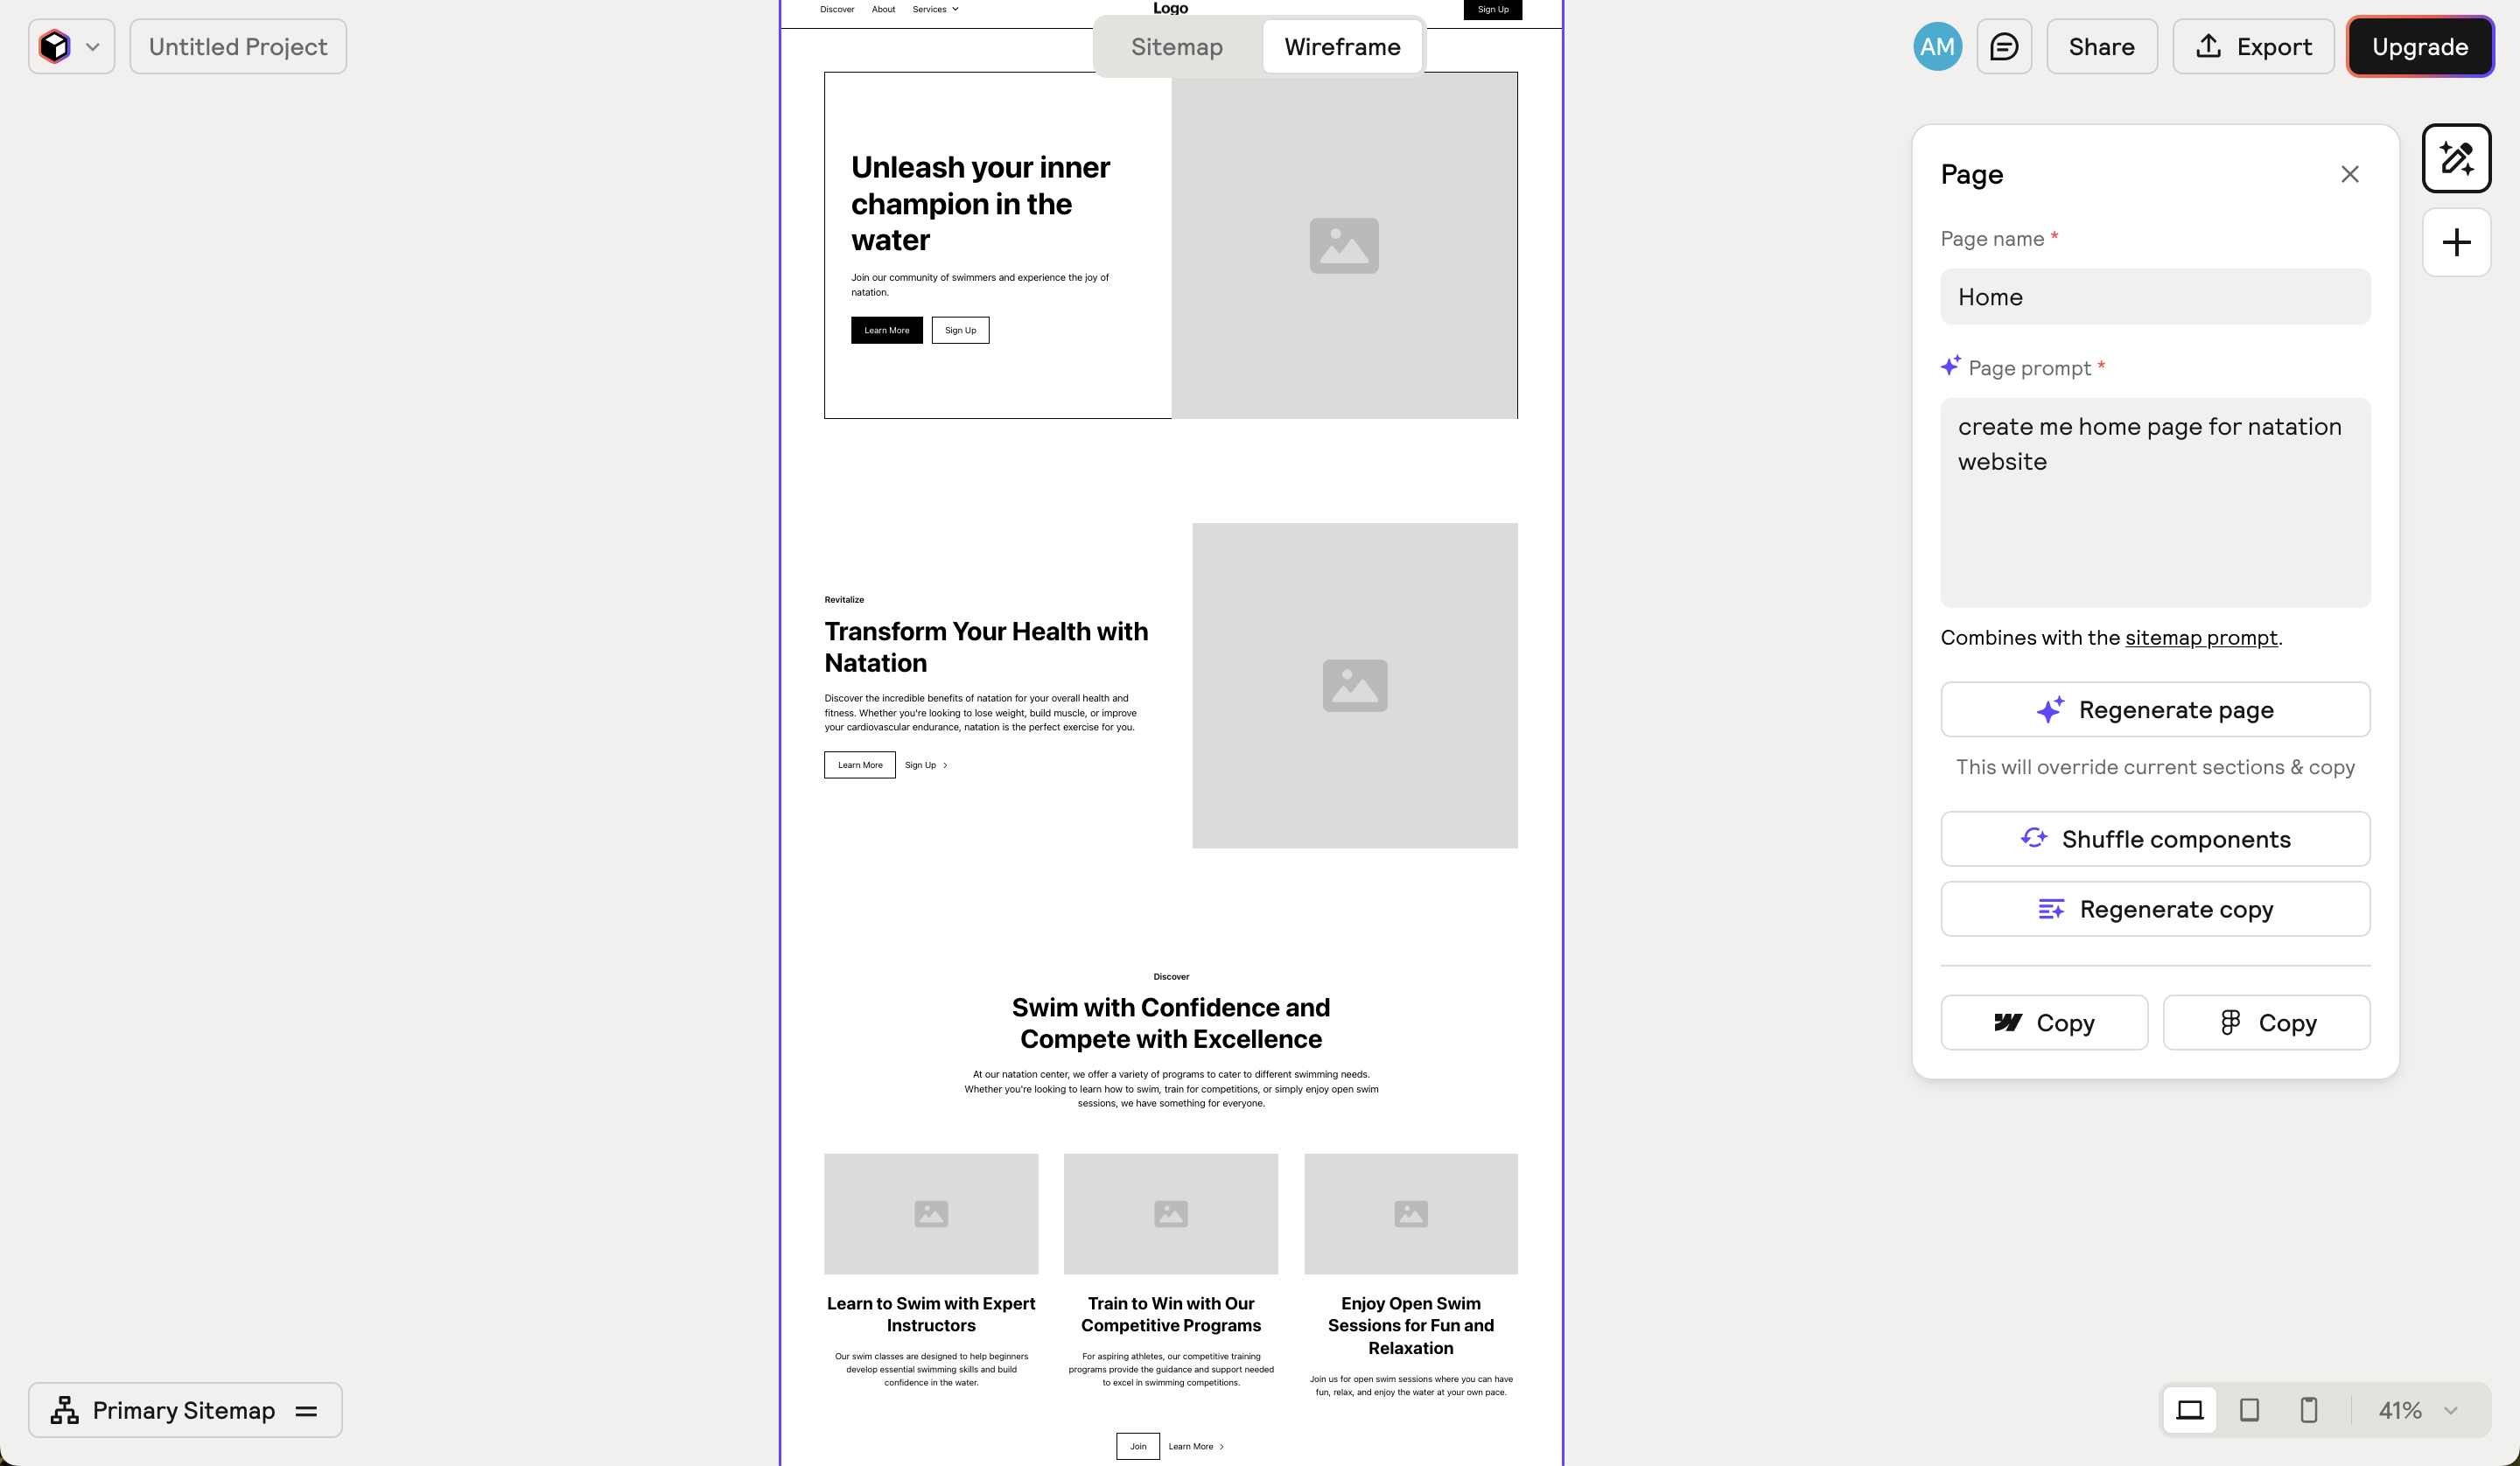
\includegraphics[width=0.8\textwidth]{Includes/Images/relume.png}
  \caption{Exemple de génération de site web sur la natation avec Relume}
  \label{fig: relume}
\end{figure} 

De plus, Relume est particulièrement efficace pour les sites classiques, comme les sites e-commerce, qui utilisent souvent des composants récurrents tels que des carrousels, des barres de navigation, des pieds de page, etc.

Nous pouvons voir un exemple d'une génération de site web sur la natation avec Relume, nous pouvons voir la structure du site, les pages et les composants générés automatiquement (voir figure \ref{fig: relume}).
C'est idéal pour les projets simples, Relume se distingue par sa capacité à augmenter la productivité tout en simplifiant la gestion des projets web. Toutefois, pour des projets plus complexes nécessitant des designs et des contenus plus personnalisés, l’intervention humaine reste indispensable. 

\subsection{Webflow}
Webflow est une plateforme innovante de conception et de développement de sites web qui permet de créer des sites professionnels sans nécessiter de compétences en codage. Intégrant un éditeur visuel intuitif, Webflow permet de concevoir et de personnaliser des pages web à l'aide de fonctionnalités de glisser-déposer, tout en appliquant des styles CSS en temps réel. Les capacités avancées d'interactions et d'animations permettent de créer des expériences utilisateur engageantes, sans écrire de code complexe. De plus, Webflow offre des possibilités de low code, permettant aux développeurs d'ajouter des fonctionnalités personnalisées à travers des snippets de code et des intégrations avec d'autres outils, enrichissant ainsi l'expérience et les capacités du site. Webflow représente ainsi une solution complète et accessible alliant design esthétique et performance technique.

\subsection{DevLink}
DevLink constitue un outil de WebFlow qui facilite l'intégration des composants créés dans WebFlow à notre code (exclusivement React). Cette fonctionnalité permet d'exporter les composants créés dans WebFlow directement en code React via une simple ligne de commande. De surcroît, elle assure la synchronisation de nos composants dans notre code avec WebFlow. Ainsi, nous sommes en mesure d'importer les composants élaborés sur WebFlow dans notre code React, et de les mettre à jour automatiquement lorsque le designer effectue des modifications depuis WebFlow. 

\subsection{Contentful}
Contentful est une plateforme de gestion de contenu (CMS headless) conçue pour répondre aux besoins des développeurs. Avec son architecture flexible basée sur le cloud et son API robuste, Contentful offre une solution de gestion de contenu, les développeurs peuvent facilement intégrer Contentful à n'importe quelle technologie frontend grâce à ses API RESTful et GraphQL. Cela permet une séparation claire entre le backend et le frontend, offrant ainsi une plus grande liberté de conception et une expérience de développement plus fluide. De plus, Contentful prend en charge la collaboration en équipe avec des fonctionnalités telles que les environnements de développement, les workflows de contenu et la gestion des droits d'accès, ce qui en fait un outil incontournable pour créer des expériences web dynamiques et évolutives.

\section{Reflexion sur les difféntes possibilité d'interactions entre les outils}
Avec l'équipe nous avons réflechie sur les difféntes possiblités d'interactions.

\subsection{Possibilité n°1 - Basique}
\begin{figure}[h] 
  \centering
  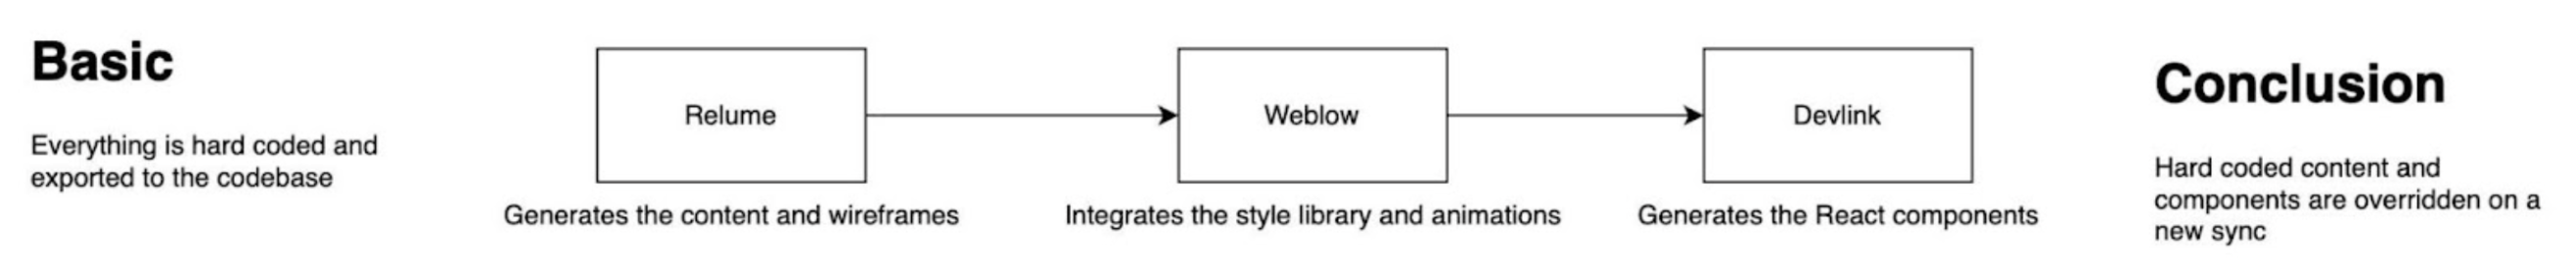
\includegraphics[width=1\textwidth]{Includes/Images/connection1.png}
  \caption{Schéma de la possibilité n°1 - Basique}
  \label{fig: Schéma de la possibilité n°1 - Basique}
\end{figure} 
La première option, la plus basique, consiste à rassembler simplement les outils (voir figure \ref{fig: Schéma de la possibilité n°1 - Basique}). Le but est de créer le site sur Relume, qui génère toute l'expérience utilisateur (UX), les wireframes, les composants et le texte. Ensuite, nous transférons tout ce que nous avons construit sur Webflow pour créer l'interface utilisateur (UI), styliser le site, ajouter des animations, etc. Enfin, avec DevLink, nous exportons tous nos composants pour les intégrer dans notre code React. Cependant, tout le texte et le contenu sont codés en dur. Si nous souhaitons modifier le texte ou les images, nous devons resynchroniser DevLink et reconstruire le site avec Next.js.

Cette méthode présente l'avantage de simplifier le processus initial de création et de design, mais elle impose des contraintes en termes de maintenance et de mises à jour de contenu. Pour chaque modification de texte ou d'image, il est nécessaire de passer par une étape de synchronisation et de reconstruction, ce qui peut être laborieux et chronophage.

\subsection{Possibilité n°2 - Avec un CMS}

Avec un CMS : L'objectif ici est de connecter Relume directement ou indirectement (via un webhook) à un CMS, afin que Relume prenne en compte le texte du CMS et l'enregistre à chaque génération. Cela permet de rendre le texte modifiable dynamiquement dans le CMS et de ne pas le perdre à chaque régénération des wireframes.

\begin{figure}[h] 
  \centering
  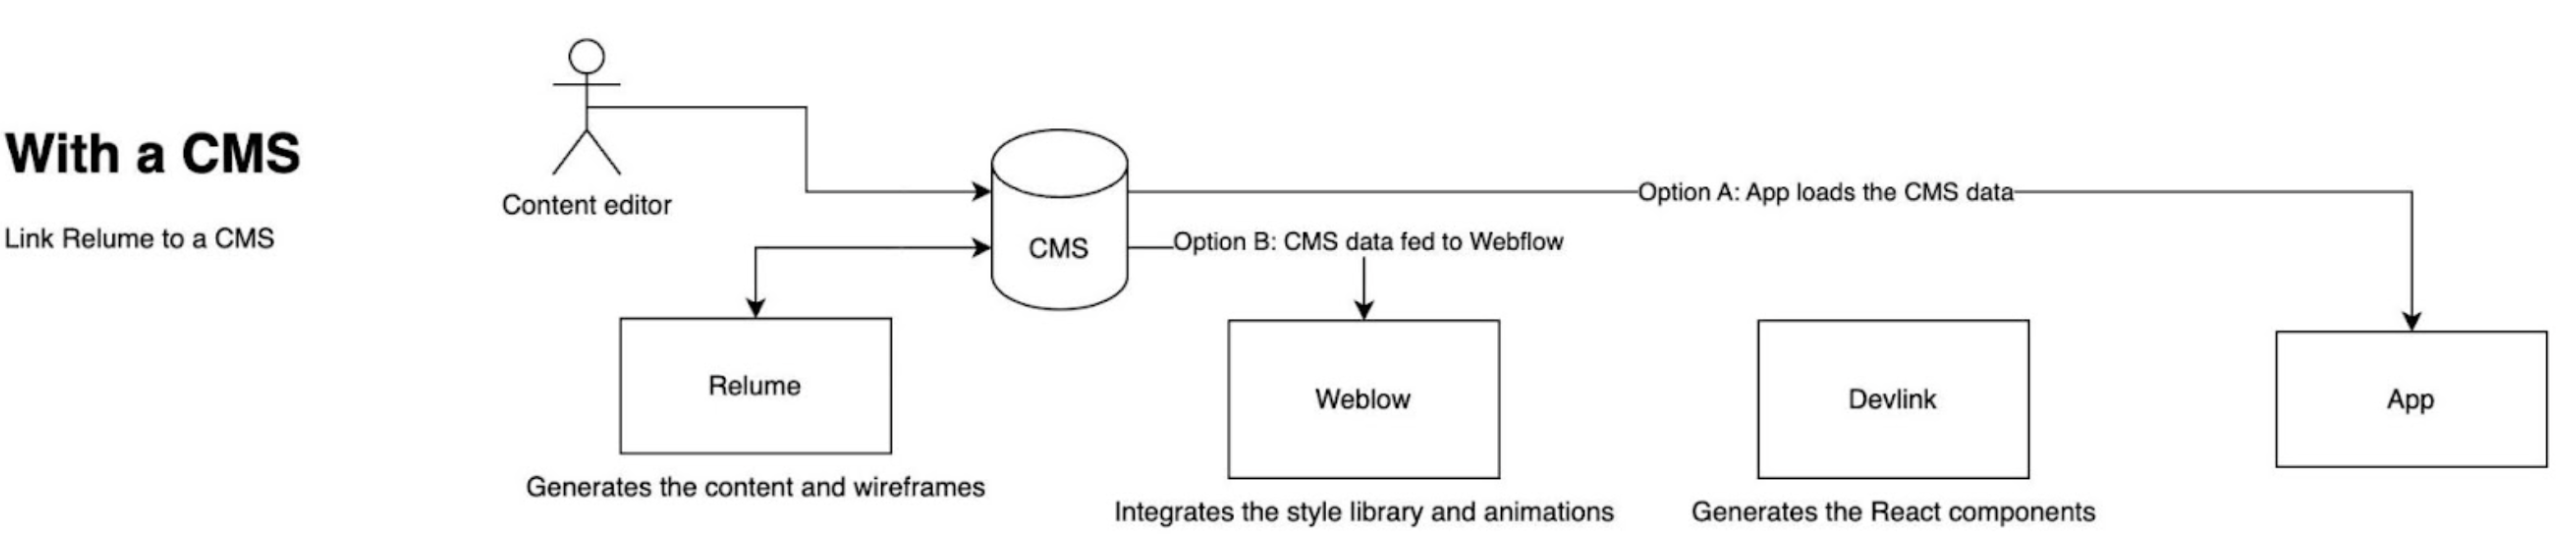
\includegraphics[width=1\textwidth]{Includes/Images/connection2.png}
  \caption{Possibilité n°2 - Avec un CMS, option A}
  \label{fig: Possibilité n°2 - Avec un CMS, option A}
\end{figure} 

Option A : Récupérer les données de la base de code React et transmettre ces données en tant que props.

\begin{figure}[h] 
  \centering
  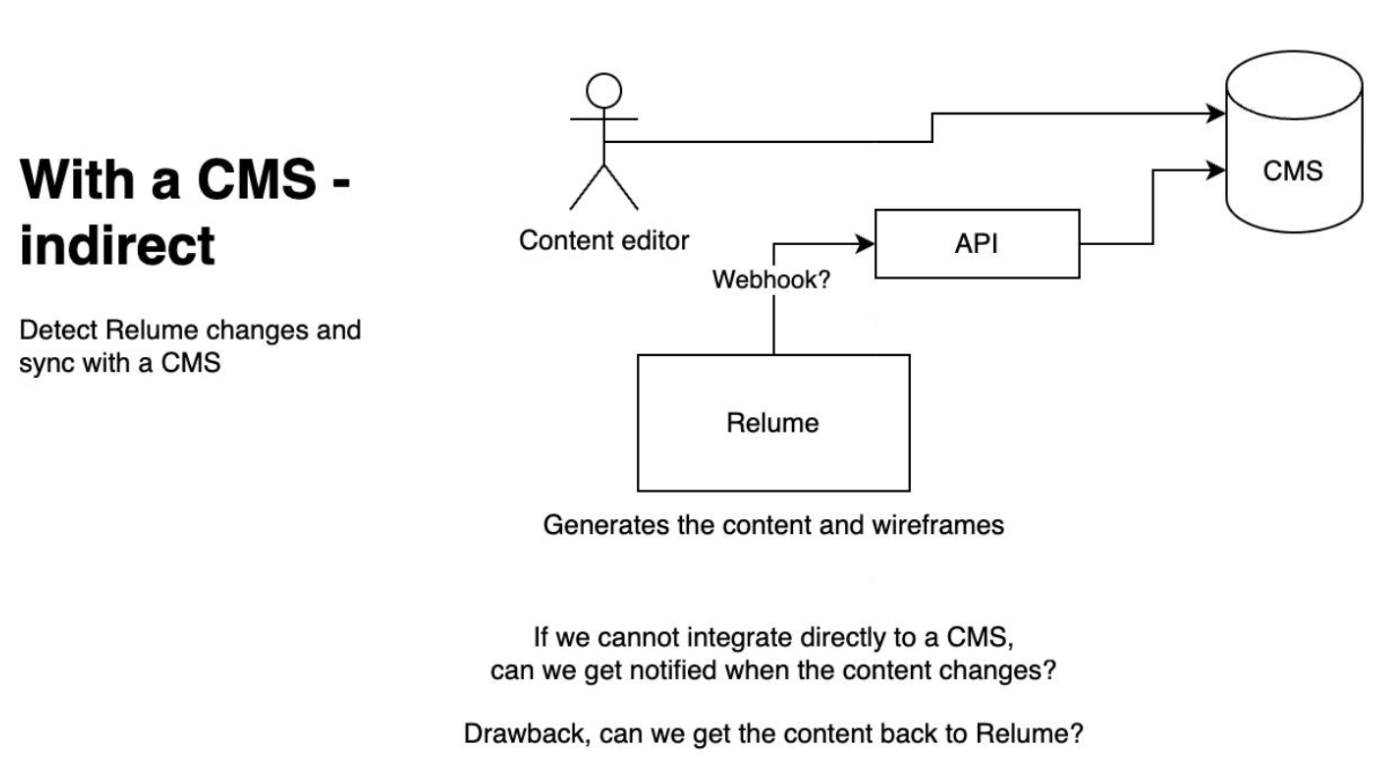
\includegraphics[width=0.6\textwidth]{Includes/Images/connection3.png}
  \caption{Possibilité n°2 - Avec un CMS, option B}
  \label{fig: Possibilité n°2 - Avec un CMS, option B}
\end{figure} 

Option B : Récupérer le texte et les données du CMS dans Webflow pour les exporter avec des données dynamiques. Cependant, cette méthode nécessiterait une nouvelle exportation à chaque fois qu'il y a un changement dans les informations.

Cette approche offre la flexibilité de modifier le contenu directement dans le CMS sans avoir à resynchroniser et reconstruire l'ensemble du site. Elle permet également de maintenir le contenu à jour plus facilement, bien que l'option B puisse impliquer des opérations supplémentaires lors de chaque modification des informations.

\section{Développement de la solution}

Nous avons commencé à développer la solution en utilisant la première option pour tester les outils et comprendre leur fonctionnement. Nous avons réussi très facilement à connecter Relume à Webflow en suivant la documentation et les tutoriels vidéo réalisés par l'équipe de Relume. DevLink, bien qu'encore en version bêta, s'est avéré facile à utiliser. Il suffit de créer un fichier de configuration \texttt{.webflowrc.js}, d'ajouter les informations de connexion à Webflow, puis de lancer la commande \texttt{npx webflow devlink sync} pour exporter et synchroniser les composants de Webflow avec React.
\\ \\
Ces outils sont très bien documentés et faciles à utiliser, ce qui nous a permis de les prendre rapidement en main. Cependant, comme mentionné précédemment, la première option présente des inconvénients en termes de maintenance et de mise à jour du contenu. C'est pourquoi nous avons décidé de nous concentrer sur la deuxième option, qui consiste à connecter Relume à un CMS pour gérer le contenu de manière dynamique.

Cette approche permet de modifier le contenu directement dans le CMS sans avoir à resynchroniser et reconstruire l'ensemble du site à chaque mise à jour. Elle améliore ainsi l'efficacité de la gestion du contenu et facilite les modifications ultérieures.
\\ \\ 
Lorsqu'on a commencé à explorer la possibilité de connecter Relume à un CMS, nous avons rencontré plusieurs difficultés. Relume est une plateforme très fermée, sans documentation officielle ni ressources en ligne pour connecter Relume à un CMS ou utiliser un WebHook. La documentation de Relume consiste principalement en vidéos YouTube, qui ne sont pas adaptées à un développement durable ni aux besoins des développeurs. Une vidéo de la chaîne officielle de Relume, intitulée « Ajout de collections CMS aux composants | Relume Library », montre comment créer des composants avec des données provenant d'un CMS, mais cette opération est effectuée depuis Webflow et non depuis Relume.

Webflow propose son propre CMS, qui est stable et fonctionne très bien. Cependant, pour connecter un CMS externe comme Strapi ou Contentful, il faut « coder » cette opération en ajoutant du code JavaScript dans Webflow. Cette méthode complique l'utilisation de l'outil pour des utilisateurs non techniques, tels que les designers graphiques.

Nous avons donc décidé de repenser notre approche pour trouver une solution plus simple et plus efficace. 

\begin{figure}[h] 
  \centering
  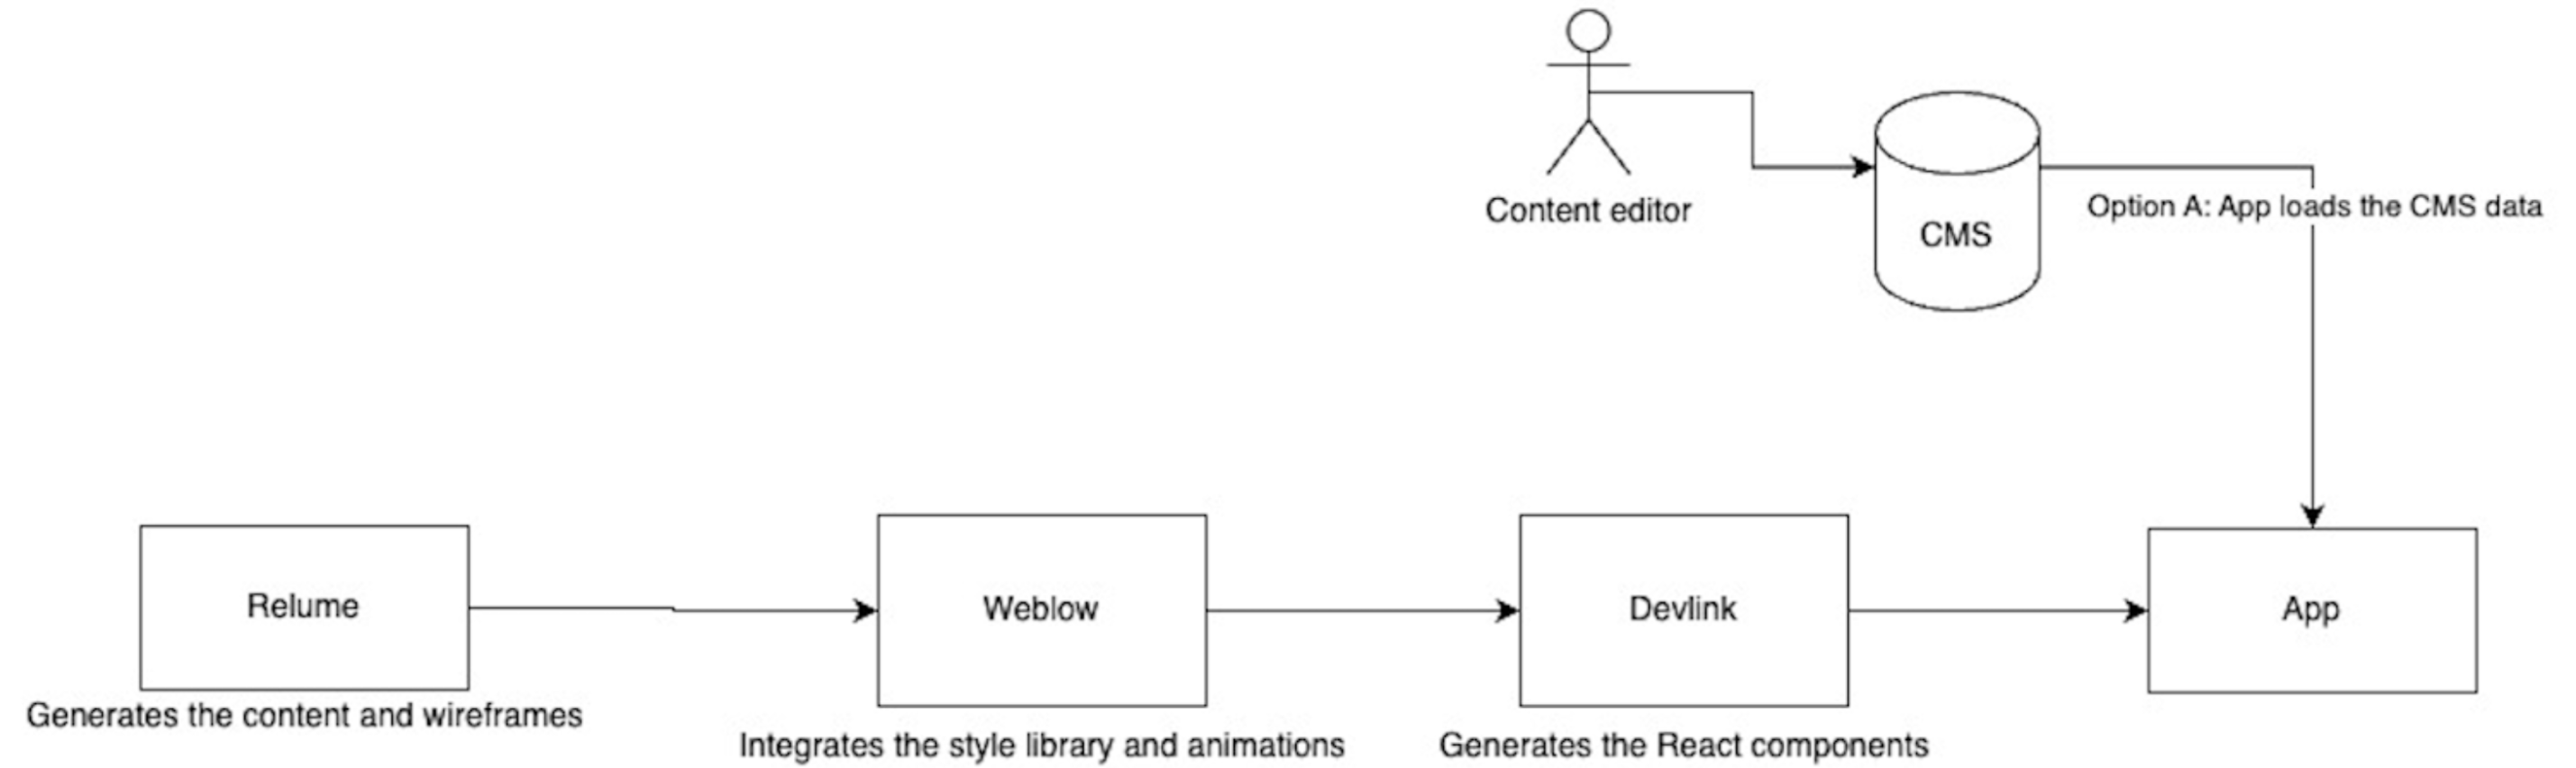
\includegraphics[width=1\textwidth]{Includes/Images/connection4.png}
  \caption{Possibilité n°3 - Avec un CMS}
  \label{fig: Possibilité n°2 - Avec un CMS}
\end{figure} 

Nous avons envisagé une nouvelle approche qui consiste à utiliser Relume pour générer les wireframes et les composants, que nous envoyons ensuite dans Webflow pour créer l'interface utilisateur (UI). Avec DevLink, nous transformons les composants Webflow en composants React et les intégrons dans notre code. Ensuite, nous connectons notre application React (Next.js) à un CMS (Contentful) pour gérer le contenu dynamique. Cette approche permet de bénéficier des avantages de chaque outil tout en simplifiant le processus de création et de gestion de contenu. Nous n'avons plus besoin de reconstruire le site à chaque modification de contenu, car nous récupérons directement le contenu du CMS en utilisant des requêtes API.

Cependant, nous devons synchroniser les composants de Webflow avec DevLink à chaque modification de ces composants et reconstruire le site pour voir les changements. Cette méthode combine la flexibilité du CMS pour la gestion dynamique du contenu avec la robustesse de Webflow et la puissance de React, tout en minimisant les efforts de maintenance.

\section{Logique de développement avec Headless CMS}
\begin{figure}[h] 
  \centering
  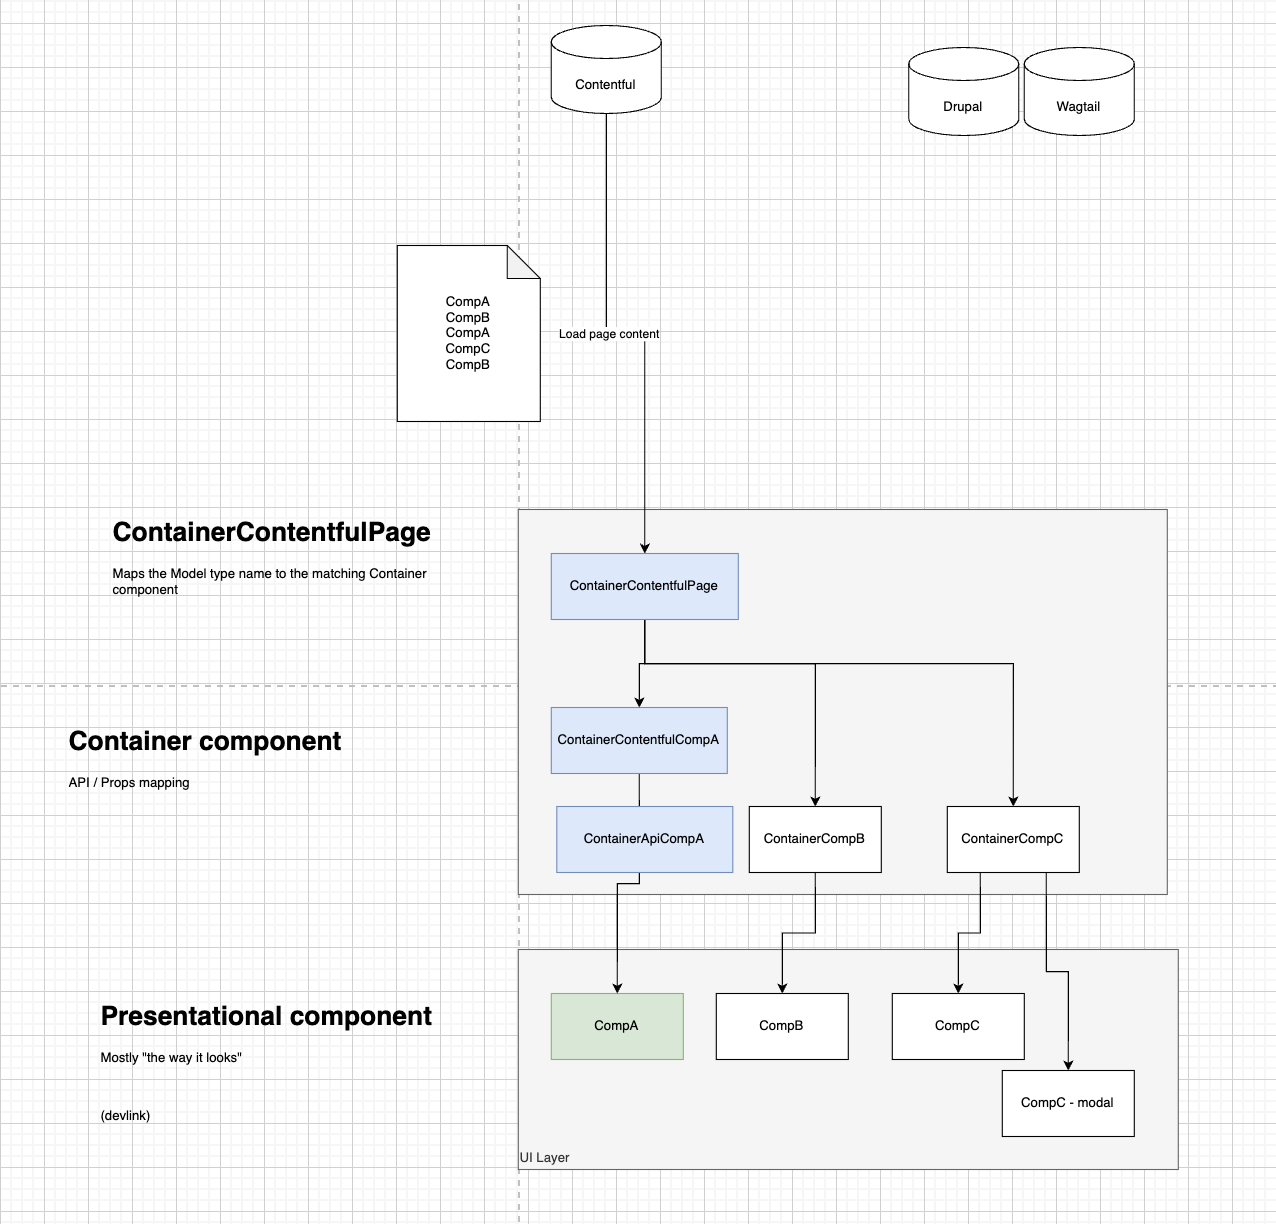
\includegraphics[width=0.93\textwidth]{Includes/Images/architecture.png}
  \caption{Architecture de la logique de développement avec Headless CMS}
  \label{fig: Architecture de la logique de développement avec Headless CMS}
\end{figure}

Pour créer la solution la plus flexible et la plus efficace possible, nous avons décidé d'utiliser un CMS headless pour gérer le contenu dynamique de notre application. Avec M. Marc Raffalli, développeur senior front-end et maître de stage, nous avons organisé plusieurs réunion pour discuter de la meilleure façon d'architecture front-end pour une connexion avec un CMS ; il m'a appris de noubreuses nouvelles façons d'apprenhender le développement front-end. La logique sous-jacente sortie de nos discussions est la suivante (voir figure \ref{fig: Architecture de la logique de développement avec Headless CMS}) :
Nous avons trois niveaux de composants.
\begin{itemize}
  \item \textbf{ContainerCMSPage}: Le but de ce component est d'implementer la logique de récupération des données d'un content type contenant les composants des pages. Le but ici est de créer la page en récupérant les composants de la page et de les afficher en donnant les props nécessaires à chaque composant.
  \item \textbf{ContainerCMSComponent}: Le but de ce composant est d'associé les données récupérer du CMS au composant Webflow.
  \item \textbf{Component}: Composant Webflow exporté avec DevLink.
\end{itemize}
\vspace{0.8cm}
Plus précisément, après avoir créer les wireframes et les composants sur Relume, styliser, animer sur Webflow et exporter les composants avec DevLink vers notre application. Nous créer des Content Type (un modèle de donnée comme un table en base de donneés) pur chaque composant, nous créeons un Content Type qui sera une liste de composants pour chaque page. Ensuite, nous récupérons les données de chaque composant de la page et les affichons dans notre application en utilisant les composants Webflow exportés.

\section{Les avantages de cette solution et les inconvénients}

Une fois le prototype de la solution développé, nous avons pu constater les avantages et les inconvénients de cette approche du point de vue techniques et fonctionnels, nous parlerons pas des avantages et des inconvénients financiers, de dépendance, de sécurité, etc.

\subsection{Avantages}
\begin{itemize}
  \item Permet de synchroniser et d'améliorer la collaboration entre les différents métiers (designers, développeurs, content managers).
  \item Le développeur front-end n'a plus besoin de s'occuper de l'implémentation du composant mais peut se concentrer sur la partie logique, l'architecture, les tests, etc.
  \item La génération du code exporté par DevLink est lisible
\end{itemize}

\subsection{Inconvénients}
\begin{itemize}
  \item Certains composants Webflow ne sont pas compatible comme la collection list, les éléments ecommerce, les animations Lottie et les lightbox.
  \item Impossibilité de modifier les composants depuis React et avoir les changements sur Webflow, la synchronisation ne fonctionne que dans un sens.
  \item L'atomic design n'est pas gérée correctement, le code généré doit être modifié mais est écrasé lors de la prochaine synchronisation.
  \item Une partie du code généré est « inutile » et peut être difficile à lire si le composant est complexe notamment avec les animations.
  \item Erreurs de synchronisation sans explication et sans gestion des erreurs.
  \item Nous avons pas trouvé de solution pour créer des props avec une structure de données personnalisée (liste, tableau, json, etc.)
\end{itemize}
